%
%  THESISBOOK
%
%  This file takes care of the (layout) definitions and groups the 
%  separate latex files to one coherent part
%
%  @author Nick Veenhof
%

\documentclass[11pt,a4paper,oneside,notitlepage]{book}

% Adjust margins
% Should be before using the package of fancyhdr
\setlength{\hoffset}{-1in}
\setlength{\voffset}{-1in}
\setlength{\topmargin}{2cm}
\setlength{\headheight}{0.5cm}
\setlength{\headsep}{1cm}
\setlength{\oddsidemargin}{3.5cm}
\setlength{\evensidemargin}{3.5cm}
\setlength{\textwidth}{16cm}
\setlength{\textheight}{23.3cm}
\setlength{\footskip}{1.5cm}

\usepackage{fancyhdr}
\usepackage{graphicx}
\usepackage{hyperref}
\usepackage[font=small,format=plain,labelfont=bf,up,textfont=normal,up,justification=justified,singlelinecheck=false]{caption}

\usepackage{listings}
\usepackage{color}
\usepackage{minted}
\usepackage{float}
\usepackage[utf8]{inputenc}
\usepackage[nonumberlist]{glossaries}
\usepackage{seqsplit}

% \makeglossaries

\pagestyle{fancy}

\renewcommand{\chaptermark}[1]{\markright{\MakeUppercase{#1}}}
\renewcommand{\sectionmark}[1]{\markright{\thesection~#1}}

\newcommand{\headerfmt}[1]{\textsl{\textsf{#1}}}
\newcommand{\headerfmtpage}[1]{\textsf{#1}}

\fancyhf{}
\fancyhead[LE,RO]{\headerfmtpage{\thepage}}
\fancyhead[LO]{\headerfmt{\rightmark}}
\fancyhead[RE]{\headerfmt{\leftmark}}
\renewcommand{\headrulewidth}{0.5pt}
\renewcommand{\footrulewidth}{0pt}

\fancypagestyle{plain}{ % First page of a chapter
  \fancyhf{}
  \fancyhead[LE,RO]{\headerfmtpage{\thepage}}
  \fancyhead[LO]{\headerfmt{\rightmark}}
  \fancyhead[RE]{\headerfmt{\leftmark}}
  \renewcommand{\headrulewidth}{0.5pt}
  \renewcommand{\footrulewidth}{0pt}
}

% 1.5 baseline (changing this will affect front page)
\renewcommand{\baselinestretch}{1.5}

\begin{document}

% \inputminted[fontsize=\scriptsize,linenos]{xml}{code_examples/schema_fieldtype.xml}

% frontpage
%  Frontpage

% Note: Uses the baseline of 1.5 that was set at the start of the book

\begin{titlepage}

\setlength{\hoffset}{-1in}
\setlength{\voffset}{-1in}
\setlength{\topmargin}{1.5cm}
\setlength{\headheight}{0.5cm}
\setlength{\headsep}{1cm}
\setlength{\oddsidemargin}{3cm}
\setlength{\evensidemargin}{3cm}
\setlength{\footskip}{1.5cm}
\enlargethispage{1cm}
% adjusting \textwidth and \textheight does not seem to work


\fontsize{12pt}{14pt}
\selectfont

\begin{center}


\includegraphics[height=5cm]{images/logoUPCblau-complet}

\vspace{0.5cm}

Barcelona School of Informatics (FIB)\\
Master in Information Technology\\

\vspace{3.5cm}

\fontseries{bx}
\fontsize{17.28pt}{21pt}
\selectfont

Improving Acquia Search and the Apache Solr Search Integration Drupal Module\\

\fontseries{m}
\fontsize{12pt}{14pt}
\selectfont

\vspace{.6cm}

by 

\vspace{.4cm}

Nick VEENHOF

\vspace{3.5cm}

Supervisor: B.~Chris BROOKINS\\
Co-Supervisor: Dr.~Ir.~Peter WOLANIN\\
Tutor/Professor: Prof.~Dr.~Carles FARR\'{E} TOST\\

\vspace{2cm}

Academic Year 2011--2012

\end{center}
\end{titlepage}


% empty page (!!)
\newpage

% No page numbering for the front page
\pagestyle{empty}

% preface with word of gratitude and license (Do not forget to sign!!)
%  Voorwoord (dankwoord) en toelating tot bruikleen

\newpage
\noindent \textbf{\huge License Statement}

\vspace{1.5cm}

\noindent
This work is licensed under the NonCommercialAcknowledgementWithoutDerivedWork license from Creative Commons. 
This license, which is the most restrictive from Creative Commons, doesn't allow derived works, and authorizes, in all cases, the reproduction, distribution and public communication of the work as long as its author is mentioned and as no commercial use is done.

\addvspace{4cm}

\noindent Nick Veenhof, February 2012


% overzicht
%  Overzichtsbladzijde met samenvatting

\newpage
{
\setlength{\baselineskip}{14pt}
\setlength{\parindent}{0pt}
\setlength{\parskip}{8pt}

\begin{center}

\noindent \textbf{\huge Improving Acquia search and the Apache Solr Module\\[8pt]}


by 

Nick VEENHOF

Master Thesis in order to acquire a Master in Information Technology

Academic Year 2011--2012

Supervisor: B.~Chris BROOKINS\\
Co-Supervisor: Dr.~Ir.~Peter WOLANIN\\
Tutor/Professor: Prof.~Dr.~Ir.~Carles FARR\'{E} TOST\\

Barcelona School of Informatics (FIB)\\
Master in Information Technology\\
BarcelonaTech

\end{center}

\section*{Abstract}

% TODO: Abstract

This work is intended to show the upgrade process of a module on drupal.org using community tools. This study was performed as part of an internship at Acquia Inc during a period of 5 months. More specifically it was focussed on creating a stable release of the Apache Solr Search Integration Module for Drupal 7 and eventually also backport this to Drupal 6. 
Firstly there was  an analysis state and a brief introduction to how the system worked and how to co-operate with an existing Open Source community. From this, existing problems were identified and thrown in a roadmap. Community projects have a very dynamic rhythm and issues could rise up or get resolved because thousands of persons had access to the code base. These challenges are described and tips are given on how to cope with such a dynamic development process.
This study also describes the challenges of a backport and how to resolve them. 
Finally, there is an explanation of the Acquia Search service and the process to upgrade the server park from Solr 1.4 to Solr 3.x (initially 3.4, finally 3.5) that includes the process of writing a Java servlet for managing authentication over rest services using RFC2104 HMAC encryption.

\section*{Keywords}
Drupal, Apache Solr, Lucene, Acquia, Acquia Search, Acquia Network, Search Technology
}

\newpage % Necessary to prevent a header to pop up on this page


\pagestyle{fancy}
\frontmatter

% Table of contents
\tableofcontents

% opmaak voor het eigenlijke boek; onderstaande lijnen
% weglaten als de eerste regel van een nieuwe alinea moet
% inspringen in plaats van extra tussenruimte
%\setlength{\parindent}{0pt}
%\setlength{\parskip}{0.5\baselineskip plus 0.5ex minus 0.2ex}
%\setlength{\parskip}{1ex plus 0.5ex minus 0.2ex}

% Chapters
\mainmatter

% Include chapters here (\includes)
% Define the glossary words
\newglossaryentry{document}{name=document,
description={A document is a sequence of fields}, plural=documents}
\newglossaryentry{field}{name=field,
description={A field is a named sequence of terms}, plural=fields}
\newglossaryentry{term}{name=term,
description={A term is a string}}


\chapter{Introduction}

\section{Web and Search}

\paragraph{}
It wouldn't be wrong to start with a quote from the famous paper of Sergey Brin and Lawrence Page. "The web creates new challenges for information retrieval. The amount of information on the web is growing rapidly, as well as the number of new users inexperienced in the art of web research. People are likely to surf the web using its link graph" \cite{google_paper}
In my personal opinion I also experienced that people "Google" more and more and this phenomenon intrigued me and many others. The web won't stop growing and content is added in amounts that we can't imagine. Even though Google does its very best to index every piece of content it still lacks in a more customizable way to find data. You, as a reader, will probably already have searched in depth in a search engine other than Google. For example, ebay.com has a very specific search engine that allows their customers to find products and goods that are are exactly what to user is searching for by narrowing down the results using Facets \footnote{A faceted classification system allows the assignment of an object to multiple characteristics (attributes), enabling the classification to be ordered in multiple ways, rather than in a single, predetermined, taxonomic order. For example, a collection of books might be classified using an author facet, a subject facet, a date facet, etc.}

Another missing piece in the search part of the global web is the ability to search in restricted content. Say, for example, an intranet can't benefit from a global search, hence a search engine that indexes content in a customized way is necessary. 

A numerous amount of projects \footnote{\url{http://en.wikipedia.org/wiki/List_of_enterprise_search_vendors} has a list with most of the current enterprise search solutions}allow you to customize the indexing process while still supporting hundreds of thousands \glspl{document} which contains \glspl{field} with customized data. Creating an application that includes integration with access permissions is not easy but it is do-able.

\section{Open Source \& Community}
\paragraph{}
This work is the result of many hours hard work and not only from myself, as the author but also from a complete community. These communities have changed the way how we look at software. In programming classes in university a student is taught a different way of designing software, the control of this process is fully his. There are numerous courses going from basic Java to Advanced Web Technologies to IBM rational rose project management in the FIB department of the UPC. While you can learn a ton from these courses it is never enough and by being an active member of a community the obligation you have to follow and participate in life-long learning is fulfilled. Every day there might be an aha-erlebnis \footnote{An insight that manifests itself suddenly, such as understanding how to solve a difficult problem, is sometimes called by the German word Aha-Erlebnis. It is also known as an epiphany.} or frustrations but in the end it is worthwhile for the personal evolution. 

Also, since this topic is about Search Applications and Web Applications we only focus on Open Source tools that help us in achieving our goals. See section \ref{chap:description} on page \pageref{chap:description} to find out more about the specifics of these tools and why these tools were chosen. 

\paragraph{}
Working in a community is, similarly, another way of creating solutions for a set of existing problems but involves a different way of making decisions and looking at software. It is great if the code that is written can be shared and is being used by thousands of people and can be corrected by those same group of people. While code will never be perfect, different people have used the same codebase to solve existing problems and they have been saving time and resources. The company where this thesis was executed, Acquia \footnote{\url{http://www.acquia.com}}, is doing an fantastic job in supporting these very necessary skills and promoting shared knowledge.

As Dries Buytaert, the man who initially built Drupal and founded Acquia, once said : 
\begin{quote}First, Open Source adoption in the enterprise is trending at an incredible rate -- Drupal adoption has grown a lot in 2009 but we saw by far the biggest relative growth in the enterprise. Fueling this movement is the notion that Open Source options present an innovative, economically friendly and more secure alternative to their costly proprietary counterparts. Second, Cloud Computing is a transformational movement in that it enables continual innovation and updating - not to mention a highly expandable infrastructure that will reduce the burden on your IT team.

It is no surprise that Acquia's strategy is closely aligned with those two trends: Drupal Gardens, Acquia Hosting and Acquia Search are all built on Open Source tools and delivered as Software as a Service in the cloud. Combining Open Source tools and Cloud Computing makes for the perfect storm for success. It provides real value to end-users and it enables companies to monetize Open Source. It creates a win-win situation. \footnote{\url{http://buytaert.net/open-source-in-the-enterprise-and-in-the-cloud}} \end{quote}

This quote mentions Acquia Search, the service that combines Apache Solr (The chosen search engine in this work) and Drupal to provide a superior search solution as a service especially focussed on integrating Drupal with Apache Solr in the Cloud. Everything that is done to improve this has also been open sourced, including this work.

Drupal and all contributed files hosted on Drupal.org are licensed under the GNU General Public License, version 2 or later. That means you are free to download, reuse, modify, and distribute any files hosted in Drupal.org's Git repositories under the terms of either the GPL version 2 or version 3, and to run Drupal in combination with any code with any license that is compatible with either versions 2 or 3, such as the Affero General Public License (AGPL) version 3. \cite{drupal_license}

Apache Solr is licensed under the Apache License 2.0. Like any free software license, the Apache License allows the user of the software the freedom to use the software for any purpose, to distribute it, to modify it, and to distribute modified versions of the software, under the terms of the license. The Apache License, like most other permissive licenses, does not require modified versions of the software to be distributed using the same license (in contrast to copyleft licenses such as the Drupal license). In every licensed file, any original copyright, patent, trademark, and attribution notices in redistributed code must be preserved (excluding notices that do not pertain to any part of the derivative works); and, in every licensed file changed, a notification must be added stating that changes have been made to that file. \cite{apache_license}

\section{Personal History}
\paragraph{}
My story with Drupal starts in the beginning of 2007. I've done my Bachelor degree at the Katholic University of Ghent\footnote{\url{http://www.kaho.be}}. During the second year of my Bachelor I was asked, together with a 2 other people, to make a community site in Drupal to see what is was capable of. This was created in Drupal 5 and while it wasn't as powerful as it is now we were already able to integrate LDAP into the website and customize it to our needs. I do have to admit that we, as a group, made numerous mistakes against the ethics of customizing Drupal back in the days. \footnote{Insert drupal code standards here} 

\paragraph{}
This Drupal 5 project ended, my bachelor ended and I started looking for a job and ended up with a small company called Krimson \footnote{\url{http://www.krimson.be}}. This company taught me the correct way of programming Drupal and Immediately they said : "You can start with Drupal 6, very new and way better compared with the previous version". And so I did, I started creating websites full of interactivity and community, backends that connect directly to databases running on a mainframe and even planted the initial bean of interest in search (Solr) that later would appear to grow out as this thesis topic. That website is still active on the address of \url{http://www.kortingsreus.nl}. It is also there that I created my first Drupal module, namely apachesolr\_ubercart \footnote{\url{http://drupal.org/project/apachesolr_ubercart}}
\paragraph{}
Afterwards I moved to Spain to study at the UPC \footnote{\url{http://www.upc.edu/}} and started to work half time at Ateneatech \footnote{\url{http://ateneatech.com/}} and later for AT-Sistemas as one of the reference engineers for a huge Solr and Drupal powered website. \footnote{\url{http://www.elsevier.es}}. Louis Toubes, one of the lead engineers, was able to give a small reference : "Nick tiene una capacidad innata de aprender por sí solo nuevas tecnologias y lo más importante es que el disfruta con ello. Sin duda, Nick es una de esas personas que desde el primer momento que la conoces sabes que aprenderás mucho de él."

\paragraph{}
During my studies at UPC I kept following the Drupal development and made numerous discussions with people and teachers on how software engineering should look at these projects. In the course of Advanced Web Technologies I even presented Drupal in classes : "Drupal as a framework" \footnote{\url{http://prezi.com/10_1ssdjroao/}}
\paragraph{}
There was only 1 logical step possible as my next step and that was doing an internship/thesis with Acquia. During my Erasmus period in Portugal I attended a Drupal Camp and I was also a presenter at the conference {\footnote{\url{http://lisboa2011.drupal-pt.org/sessoes/apachesolr-the-complete-search-solution}} and I've met Robert Douglas, one of the creators of the Apache Solr Integration Project for Drupal and approached him with the question if I would be able to do my internship with Acquia. After a long process with the UPC and with Acquia everything was set and the pieces of the puzzle fell in place.
\paragraph{}
Now,  being 2012 and a couple of years later I still don't fully know what Drupal and all its derivatives are capable of since it keeps evolving and growing. And that's good because it keeps me as a person growing and it keeps me up to date with most of the latest web technologies. This work is a piece in the puzzle I tried to make during my short time involved with these concepts. 

\chapter{Objectives}
\paragraph{}
The student will be asked to be on-site at the headquarters in Boston for a couple of weeks in order to meet the team and to get to know the company in order to gather all the information necessary to reach the objectives set further in this document. He will follow and join meetings to obtain a good insight in the requirements of the project and learn how to work under a Agile/Scrum based development methodology.

\paragraph{}
Being responsible for improving the Drupal Apache Solr search integration [1] project and the Acquia Search service is the common theme of the whole internship. This means adding additional features, keeping high quality and create upgrades and updates. The objective will be to exploit as much as possible from the latest Apache Solr 3.x branch while merging and keeping the software compatible with Apache Solr 1.4.

\paragraph{}
Communication will be a crucial part in order to succeed. The project has a worldwide scope, reaching out to more companies then just Acquia. This means he will have to be able to consult and make decisions after talking with a lot of end-users and other stakeholders. English will be the language of choice. This can happen by means of chat (IRC), on the Drupal community website \cite{drupal_site}, giving presentations in conferences or taking interviews.
Finally the ability to work remotely, over a large distance and in a team, is an important skill to acquire.

\paragraph{Roadmap}
\begin{itemize}
  \item Bring Apache Solr \cite{apachesolr_project} for Drupal 7 to a stable Release Candidate.
  \item Bring Facet Api \cite{facetapi_project} for Drupal 7 to a stable Release Candidate.
  \item Update the Acquia Search service \cite{acquia_search} to the latest stable Apache Solr version. Upgrade the custom java code that was written to be able to authenticate customers.
  \item Backport to a new Drupal 6 branch all the new features that have been programmed into the Drupal 7 version of the Apache Solr Search Integration Module. This includes the backporting of the multisite module.
  \item Achieve mastery of the agile/scrum process, the open source software engineering methods, and the team communication processes used by Acquia.
  \item Empower the community to use the Apache Solr Search Integration project by means of Presentations, Blog posts and other interactions with community members.
  \item Create a multisite module to search between 2 or more Drupal sites or integrate this into the existing modules.  
 \end{itemize}
\chapter{Description}
\label{chap:description}
This chapter gives a short overview of technical concepts used in this work. It is not intended
to be exhaustive and references are given for further reading

\section{Acquia}
\paragraph{} 
Acquia is a commercial open source software company providing products, services, and technical support for the open source Drupal social publishing system and was founded by Dries Buytaert, the original creator and project lead of the Drupal project. With over two million downloads since inception, Drupal is used by web developers worldwide to build sophisticated community websites. Diverse organizations use Drupal as their core social publishing system for external facing websites and internal collaboration applications.

\paragraph{}
Acquia Search\footnote{\url{http://acquia.com/products-services/acquia-search}} is a plug-and-play service within the Acquia Network \footnote{\url{http://www.acquia.com/products-services/acquia-network}}, built on Apache Solr \footnote{\url{http://drupal.org/project/apachesolr}} and is available for any Drupal 6 or Drupal 7 site. Acquia Search offers site visitors faceted search navigation and content recommendations to help them find valuable information faster. It is a fully redundant, high performance cloud service, with no software to install or servers to manage.

\section{Apache Solr}
\paragraph{}
Apache Solr is an open source enterprise search platform created on top of the Apache Lucene project. Its major features include powerful full-text search, hit highlighting, faceted search, dynamic clustering, database integration, and rich document (e.g., Word, PDF) handling. Providing distributed search and index replication, Solr is highly scalable.

\paragraph{}
Apache Solr is written in Java and runs as a standalone full-text search server within a servlet container such as Apache Tomcat. Solr uses the Lucene Java search library at its core for full-text indexing and search, and has REST-like HTTP/XML and JSON APIs that make it easy to use from virtually any programming language. 
\paragraph{}
Solr's powerful external configuration allows it to be tailored to almost any type of application without Java coding, and it has an extensive plugin architecture when more advanced customization is required. Further in this work you can find an example of such a plugin written to provide extra functionality for Acquia.
\paragraph{}
When looking at a Lucene index, compared to a relational database, it seems that the index is one database table and has very fast lookups and different specific filters for text search. It takes time to create an index like this. Solr adds a front-end to the Lucene backend and many other additions.
\paragraph{}
Fundamentally, Solr is very simple. One feeds it with information (documents) and afterwards you query Solr and receive the documents that match the query. Solr allows applications to build indexes based on different fields\footnote{Fields are different kinds of entries}. These fields are defined in a schema which tells Solr how it should build the index.

Using analyzers and tokenizers a search query is processed. Field analyzers are used both during ingestion, when a document is indexed, and at query time. An analyzer examines the text of fields and generates a token stream. Analyzers may be a single class or they may be composed of a series of tokenizer and filter classes.

Tokenizers break field data into lexical units, or tokens. Filters examine a stream of tokens and keep them, transform or discard them, or create new ones. Tokenizers and filters may be combined to form pipelines, or chains, where the output of one is input to the next. Such a sequence of tokenizers and filters is called an analyzer and the resulting output of an analyzer is used to match query results or build indices.

Although the analysis process is used for both indexing and querying, the same analysis process need not be used for both operations. For indexing, you often want to simplify, or normalize, words. For example, setting all letters to lowercase, eliminating punctuation and accents, mapping words to their stems, and so on. Doing so can increase recall because, for example, "ram", "Ram" and "RAM" would all match a query for "ram". To increase query-time precision, a filter could be employed to narrow the matches by, for example, ignoring all-cap acronyms if you're interested in male sheep, but not Random Access Memory.

The tokens output by the analysis process define the values, or terms, of that field and are used either to build an index of those terms when a new document is added, or to identify which documents contain the terms your are querying for.

\section{Drupal}
\paragraph{History}
Drupal is originally written by Dries Buytaert as a message board. It became an open source project in 2001. Drupal is a free and open-source content management system (CMS) written in PHP and distributed under the GNU General Public License. It is used as a back-end system for at least 1.5\% of all websites worldwide ranging from personal blogs to corporate, political, and government sites including whitehouse.gov and data.gov.uk. It is also used for knowledge management and business collaboration.

\paragraph{}
The standard release of Drupal, known as Drupal core, contains basic features common to content management systems. These include user account registration and maintenance, menu management, RSS-feeds, page layout customization, system administrationand even a basic search functionalty. The Drupal core installation can be used as a brochureware website, a single- or multi-user blog, an Internet forum, or a community website providing for user-generated content.

\paragraph{Basic understanding}
A single web site could contain many types of content, such as informational pages, news items, polls, blog posts, real estate listings, etc. In Drupal, each item of content is called a node (internally called an entity), and each node belongs to a single content type (internally called entity type), which defines various default settings for nodes of that type, such as whether the node is published automatically and whether comments are permitted. (Note that in versions below 7 of Drupal, content types were known as node types.)

\paragraph{Contributed Modules}
There are more than 12,000 free community-contributed addons, known as contrib modules, available to alter and extend Drupal's core capabilities and add new features or customize Drupal's behavior and appearance. Because of this plug-in extensibility and modular design, Drupal is sometimes described as a content management framework. Drupal is also described as a web application framework, as it meets the generally accepted feature requirements for such frameworks.
While Drupal core (7) comes with advanced search capabilities it is still restricted by regular databases. \footnote{Any database that is compliant with the SQL standard should be able to run Drupal 7}. The module that was created during this work is also defined as a contributed module.

\paragraph{Apache Solr Search Integration}
The Drupal module integrates Drupal with the Apache Solr search platform. Faceted search is supported if the facet API module is used. Facets will be available for you ranging from content author to taxonomy to arbitrary fields. The module also includes functionalities such as :
\begin{itemize}
  \item Search pages, eg.: multiple search pages with optionally customized search results.
  \item Multiple environments to support multiple Solr servers.
  \item Comes with support for the node content type including dynamic fields.
  \item Can override the taxonomy pages and use output from Solr to generate taxonomy overview pages.
  \item Can override the user content listing pages using output from Solr to generate these.
  \item Custom Content types (entities) indexing through hooks.
  \item Add biases and boosts to specific fields or content types
  \item Range Query type, that in combination with facet API and Facet Api Slider a very rich faceting experience delivers to the end user.
  \item Supports a lot of customizations without having to modify the source code
\end{itemize}




\chapter{Exploration}
This chapter describes the process of the index concepts in Apache Solr, explains how the Apache Solr Search Integration module for Drupal works when indexing and points out some of the improvements that should be made. It also takes a deeper look in the Facet Api \footnote{\url{http://www.drupal.org/project/facetapi}}module to see how it is structured and where it could use improvements. And finally a brief analysis for the upgrade from Apache Solr 1.4 to Apache Solr 3.5 in the context of Acquia Search service.

\section{Apache Solr}
\paragraph{Version conflicts}
Apache Solr consists out of a number of parts. The analysis part tries to explain you all it entails. When Drupal 6 came out and became popular, there was only one version of Apache Solr available. This was version 1.4 and was not yet merged with the Lucene branch. Solr's version number was synced with Lucene following the Lucene/Solr merge, so Solr 3.1 contains Lucene 3.1. Solr 3.1 is the first release after Solr 1.4.1. All the explanation that follows will be for Solr 3.x since this is the version that is used and was aimed at during the creation of this project.

\paragraph{Fields}
There are different field types defined in the original schema.xml that used to come with the module. A field type has four types of information. Most of this information is gathered from \cite{solr3} and \cite{solr14}.
\begin{itemize}
  \item The name of the field type
  \item An implementation class name
  \item If the field type is TextField, a description of the field analysis for the field type
  \item Field attributes
\end{itemize}
To illustrate this there is listing \ref{code:fieldtypedefinition} as an example of a field type definition as it is used in the schema provided with the Apache Solr Module and also a list of all possible field types in listing \ref{lst:fieldtypedefinition}.

\begin{longtable}{| p{4cm} | p{11cm} |}
    \hline
    Class & Description \\ \hline
    BCDIntField & Binary-coded decimal (BCD) integer. BCD is a relatively inefficient 
    encoding algorithm that offers the benefits of quick decimal calculations and quick conversion to a string. \\ \hline
    BCDLongField & BCD long integer \\ \hline
    BCDStrField & BCD string \\ \hline
    *BinaryField & Binary data \\ \hline
    *BoolField & Contains either true or false. Values of "1", "t", or "T" in the first character are interpreted as true. Any other values in the first character are interpreted as false. \\ \hline
    ByteField & Contains an array of bytes. \\ \hline
    *DateField & Represents a point in time with millisecond precision. \\ \hline
    DoubleField & Double (64-bit IEEE floating point) \\ \hline
    ExternalFileField & Pulls values from a file on disk. \\ \hline
    FloatField & Floating point (32-bit IEEE floating point) \\ \hline
    IntField & Integer (32-bit signed integer) \\ \hline
    LongField & Long integer (64-bit signed integer) \\ \hline
    *RandomSortField & Does not contain a value. Queries that sort on this field type will return results in random order. Use a dynamic field to use this feature. \\ \hline
    ShortField & Short integer \\ \hline
    SortableDoubleField & The Sortable* fields provide correct numeric sorting. If you use the plain types (DoubleField, IntField, and so on) sorting will be lexicographical instead of numeric. \\ \hline
    SortableFloatField & Numerically sorted floating point \\ \hline
    SortableIntField & Numerically sorted integer \\ \hline
    SortableLongField & Numerically sorted long integer \\ \hline
    *StrField & String (UTF-8 encoded string or Unicode) \\ \hline
    *TextField & Text, usually multiple words or tokens \\ \hline
    *TrieDateField & Date field accessible for Lucene TrieRange processing \\ \hline
    *TrieDoubleField & Double field accessible Lucene TrieRange processing \\ \hline
    TrieField & If this type is used, a "type" attribute must also be specified, with a value of either: integer, long, float, double, date. Using this field is the same as using any of the Trie*Fields. \\ \hline
    *TrieFloatField & Floating point field accessible Lucene TrieRange processing \\ \hline
    *TrieIntField & Int field accessible Lucene TrieRange processing \\ \hline
    *TrieLongField & Long field accessible Lucene TrieRange processing \\ \hline
    *PointType & For spatial search: An arbitrary n-dimensional point, useful for searching sources such as blueprints or CAD drawings. \\ \hline
    *LatLonType &  Latitude/Longitude as a 2 dimensional point. Latitude is always specified first.\\ \hline
    *GeoHashField & Representing a Geohash\footnote{Geohash is a defined standard. More on wikipedia : \url{http://en.wikipedia.org/wiki/Geohash}} field. The field is provided as a lat/lon pair and is internally represented as a string.\\ \hline
    UUIDField & Universally Unique Identifier (UUID). Pass in a value of "NEW" and Solr will create a new UUID. \\ 
     \hline
\end{longtable}
\captionof{listing}{All field type definitions. Marked with a star are the ones that are used in the Apache Solr Search Integration module for Drupal  \label{lst:fieldtypedefinition}}

\paragraph{Field properties}
Important to know is that each of these fields that is shown in listing \ref{lst:fieldtypedefinition} have configurable values. Drupal uses these properties to map different dynamic fields to specific types with specific configurations. 
These dynamic fields are what we call fields from the Field API (Drupal 7) or from the Content Construction Kit (CCK, Drupal 6). With these modules it is possible to add different fields to content types\footnote{Content types are a way of defining structured data that will be inputted by users}

\begin{longtable}{| p{4.5cm} | p{8.5cm} | p{2cm} |}
    \hline
    Field Property & Description & Values \\ \hline
    indexed & If true, the value of the field can be used in queries to retrieve matching documents & true or false\\ \hline
    stored &  If true, the actual value of the field can be retrieved by queries & true or false\\ \hline
    sortMissingFirst / sortMissingLast & Control the placement of documents when a sort field is not present. As of Solr 3.5, these work for all numeric fields, including Trie and date fields. & true or false\\ \hline
    multiValued & If true, indicates that a single document might contain multiple values for this field type & true or false\\ \hline
    positionIncrementGap & For multivalued fields, specifies a distance between multiple values, which prevents spurious phrase matches & integer\\ \hline
    omitNorms & If true, omits the norms associated with this field (this disables length normalization and index-time boosting for the field, and saves some memory). Only full-text fields or fields that need an index-time boost need norms. & true or false\\ \hline
    omitTermFreqAndPositions & If true, omits term frequency, positions, and payloads from postings for this field. This can be a performance boost for fields that don't require that information. It also reduces the storage space required for the index. Queries that rely on position that are issued on a field with this option will silently fail to find documents. This property defaults to true for all fields that are not text fields. & true or false\\ \hline
    autoGeneratePhraseQueries & For text fields. If true, Solr automatically generates phrase queries for adjacent terms. If false, terms must be enclosed in double-quotes to be treated as phrases. & true or false\\ \hline
\end{longtable}
\captionof{listing}{Field type properties and their respective explanation \label{lst:fieldtypeproperties}}    

\newpage
% Code snippet of a field
\inputminted[fontsize=\scriptsize,linenos]{xml}{./code_examples/schema_fieldtype.xml}
\captionof{listing}{Example of a text field type definition \label{code:fieldtypedefinition}}

\paragraph{Analyzers, Filters and Tokenizers used by Apache Solr Search Integration}
In the snippet of the text field type definition there are some unexplained entries. Filters, tokenizers and analyzers are used to process a value submitted by the application and to be saved properly into Solr so we optimize the content for faster search. In chapter 3 these concepts were shortly explained and what follows will be a list of analyzers, tokenizers and filters used in the Drupal module. Please note that these concepts can be used during query time and also at the index time.
A complete list of the supported classes can be found at \url{http://wiki.apache.org/solr/AnalyzersTokenizersTokenFilters}.

\paragraph{}

\paragraph{WhitespaceTokenizerFactory} Simple tokenizer that splits the text stream on whitespace and returns sequences of non-whitespace characters as tokens. Note that any punctuation will be included in the tokenization. Does not ship with any arguments.
\begin{minted}[fontsize=\scriptsize,linenos]{xml}
<tokenizer class="solr.WhitespaceTokenizerFactory"/>
\end{minted}
\mbox{} \\
\mbox{} \\
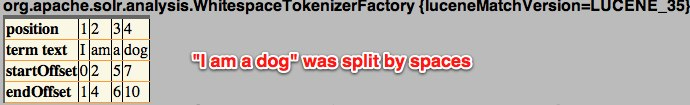
\includegraphics[width=\textwidth]{images/whitespacetokenizerfactory.jpg}

\paragraph{KeywordTokenizerFactory} Treats the entire field as a single token, regardless of its content.
\begin{minted}[fontsize=\scriptsize,linenos]{xml}
<tokenizer class="solr.KeywordTokenizerFactory"/>
\end{minted}

\paragraph{MappingCharFilterFactory} Maps Special characters to their plain equivalent
\begin{minted}[fontsize=\scriptsize,linenos]{xml}
<charFilter class="solr.MappingCharFilterFactory" mapping="mapping-ISOLatin1Accent.txt"/>
\end{minted}
Example (index time): Me alegro de que tú sonrías – It makes me happy that you smile.
\mbox{} \\
\mbox{} \\
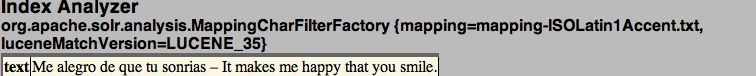
\includegraphics[width=\textwidth]{images/mappingcharfilterfactory.jpg}

\paragraph{LowerCaseFilterFactory} Lowercases the letters in each token. Leaves non-letter tokens alone. 
\begin{minted}[fontsize=\scriptsize,linenos]{xml}
<filter class="solr.LowerCaseFilterFactory"/>
\end{minted}
Example (index time): "I.B.M.", "Solr" ==> "i.b.m.", "solr".
\mbox{} \\
\mbox{} \\
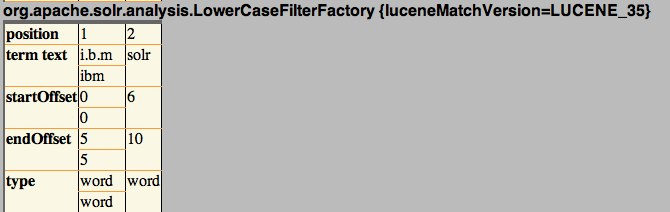
\includegraphics[width=\textwidth]{images/lowercasefilterfactory.jpg}

\paragraph{StopFilterFactory} Discards common words that are listed in the stopwords.txt file. This file is shipped in the module. Examples of these words are "an, and, are, ...". And as seen in the example it ships with some configuration options such as ignoring the case of the text and the file from where to read the stopwords from. This should be a path starting from the conf folder.  When enablePositionIncrements is true a token is stopped (discarded) and the position of the following token is incremented. This is useful if you want to know if certain words were discarded by looking at the token position.
\begin{minted}[fontsize=\scriptsize,linenos]{xml}
<filter class="solr.StopFilterFactory"
    ignoreCase="true"
    words="stopwords.txt"
    enablePositionIncrements="true"/>
\end{minted}
\inputminted[fontsize=\scriptsize,linenos]{xml}{./code_examples/stopwords.txt}
\captionof{listing}{Example of the stopwords file \label{code:stopwordsdefinition}}
Example (index time): Si Hola estoy nick a on
\mbox{} \\
\mbox{} \\
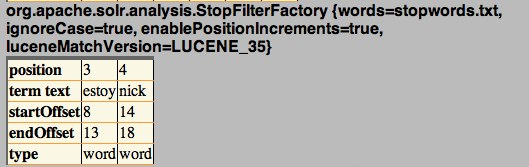
\includegraphics[width=\textwidth]{images/stopfilterfactory.jpg}

\paragraph{WordDelimiterFilterFactory} Delimits words based on parts of words. Was originally defined for the use in English based texts. It follows the following strict order but allows a number of configurations to happen. The original filter has more options but below are only the ones used in the Apache Solr schema.xml
\begin{itemize}
\item{protected} (optional) The pathname of a file that contains a list of protected words that should be passed though without splitting. In the case of Drupal these are predefined as some html entities.
\item{generateWordParts} splits words at delimiters. 
\item{generateNumberParts}  splits numeric strings at delimiters
\item{catenateWords} maximal runs of word parts will be joined: "hot-spot-sensor's" -> "hotspotsensor"
\item{catenateNumbers} maximal runs of number parts will be joined: 1947-32" -> "194732"
\item{catenateAll} Set at 0, runs of word and number parts will not be joined: "Zap-Master-9000" -> "Zap Master 9000"
\item{splitOnCaseChange} words are not split on camel-case changes:"BugBlaster-XL" -> "BugBlaster", "XL"
\item{preserveOriginal} the original token is preserved: "Zap-Master-9000" -> "Zap-Master-9000", "Zap", "Master", "9000"
\end{itemize}
\begin{minted}[fontsize=\scriptsize,linenos]{xml}
<filter class="solr.WordDelimiterFilterFactory"
    protected="protwords.txt"
    generateWordParts="1"
    generateNumberParts="1"
    catenateWords="1"
    catenateNumbers="1"
    catenateAll="0"
    splitOnCaseChange="1"
    preserveOriginal="1"/>
\end{minted}
Example text (index time): Zap-Master-9000 9000-12 BugBlaster-XL hot-spot-sensor's
\mbox{} \\
\mbox{} \\
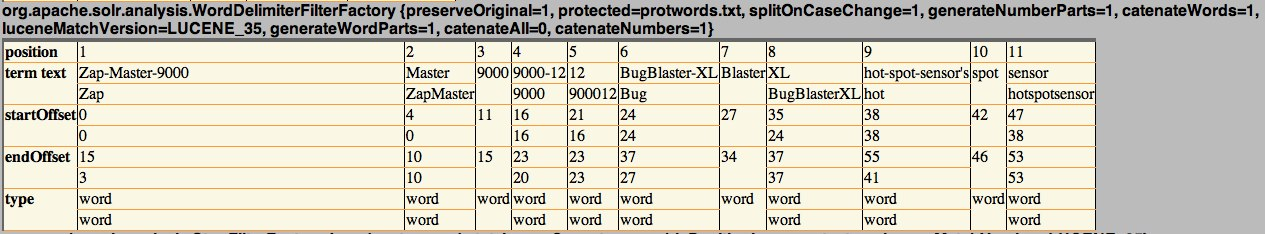
\includegraphics[width=\textwidth]{images/worddelimiterfactory.jpg}

\paragraph{LengthFilterFactory} Words smaller than 2 chars and bigger than 100 will be discarded. This is useful to speed up the query process because a blog posting from Large Scale Search with Solr mentions that a query will exponentially grow in query time when small words are used \footnote{\url{http://www.hathitrust.org/blogs/large-scale-search}}
\begin{minted}[fontsize=\scriptsize,linenos]{xml}
<filter class="solr.LengthFilterFactory" min="2" max="100" />
\end{minted}
Example Text (index time): I am a dog a b c 123
 \seqsplit{iamawordoveronehundredcharactersiamawordoveronehundredcharactersiamawordoveronehundredcharactersiamawordoveronehundredcharactersiamawordoveronehundredcharactersiamawordoveronehundredcharacters}
\mbox{} \\
\mbox{} \\
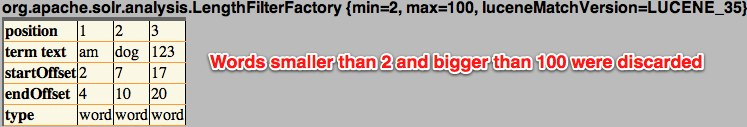
\includegraphics[width=\textwidth]{images/lengthfilterfactory.jpg}

\paragraph{SynonymFilterFactory} This is quite a special one that is only executed during query time. Meaning that words will not be processed as synonyms in index time. If a user would type color it could also check the index for texts with the word "colour". Same is valid for the more concrete example "GB,gib,gigabyte,gigabytes"
\begin{minted}[fontsize=\scriptsize,linenos]{xml}
<filter class="solr.SynonymFilterFactory" synonyms="synonyms.txt" ignoreCase="true" expand="true"/>
\end{minted}
Example Text (query time): colour test
\mbox{} \\
\mbox{} \\
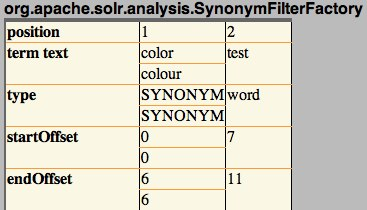
\includegraphics[width=\textwidth/2]{images/synonymfilterfactory.jpg}

\paragraph{TrimFilterFactory} This filter trims leading and/or trailing whitespace from tokens. In Drupal usecase this is used for sortable text such as names or labels. The big difference with most other filters is that this filter does not break words on spaces.
\begin{minted}[fontsize=\scriptsize,linenos]{xml}
<filter class="solr.TrimFilterFactory" />
\end{minted}
Example Text (query time): Nick Veenhof
\mbox{} \\
\mbox{} \\
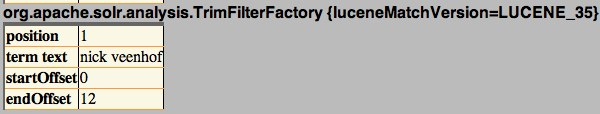
\includegraphics[width=\textwidth]{images/trimfilterfactory.jpg}

\paragraph{EdgeNGramFilterFactory} This filter generates edge n-gram tokens of sizes within the given range. In the module it was configured to return 2-gram tokens till 25-gram tokens. Especially useful for matching against queries with results. \footnote{\url{http://www.lucidimagination.com/blog/2009/09/08/auto-suggest-from-popular-queries-using-edgengrams/}}
\begin{minted}[fontsize=\scriptsize,linenos]{xml}
<filter class="solr.EdgeNGramFilterFactory" minGramSize="2" maxGramSize="25" />
\end{minted}
Example Text (index time) : I am a dog with a longbigtext
\mbox{} \\
\mbox{} \\
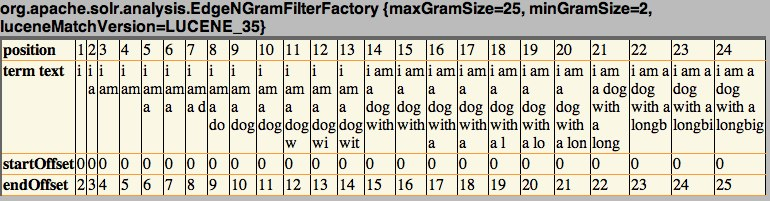
\includegraphics[width=\textwidth]{images/edgengramfilterfactory.jpg}

\paragraph{SnowballPorterFilterFactory} Snowball is a software package that generates pattern-based word stemmers. It works efficiently and fast and one can configure the language that is preferred. Apache Solr comes with a whole range of languages. English is very well supported but also Catalan and Spanish. A list of all the languages can be found in the documentation of Apache Solr or in the Snowball website \footnote{\url{http://snowball.tartarus.org/}}. Also interesting to note is that there is a file called protwords.txt (Protected words) where you can define strings that won't be stemmed.
\begin{minted}[fontsize=\scriptsize,linenos]{xml}
<filter class="solr.SnowballPorterFilterFactory" language="English" protected="protwords.txt"/>
\end{minted}
Example Text (index time) : football footballing
\mbox{} \\
\mbox{} \\
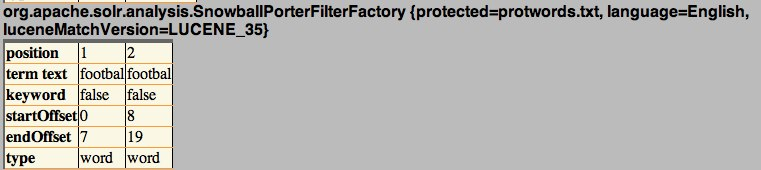
\includegraphics[width=\textwidth]{images/snowballporterfilterfactory.jpg}

\paragraph{RemoveDuplicatesTokenFilterFactory} Removes duplicates from the query or the index value.
\begin{minted}[fontsize=\scriptsize,linenos]{xml}
<filter class="solr.RemoveDuplicatesTokenFilterFactory"/>
\end{minted}
Example : Nick Nick Nick

\paragraph{Speed} Speed is an important factor. During the research phase I found an interesting article \footnote{\url{http://www.hathitrust.org/blogs/large-scale-search/slow-queries-and-common-words-part-1}} that showed a graph of the response time for their index. 
This graph shows that 97\% of the requests were completed in less than a second. The average was found to be 673 milliseconds. Those 3\% of the queries are slower because there is a longer disk seek time. This means that some queries contains commonly occurring words such as "a", "of", "the", "and", etc... Queries with common words take longer because the data structures containing the lists of documents containing those words in the index are larger.
This same source mentions that the common\-grams filter \footnote{\url{http://wiki.apache.org/solr/AnalyzersTokenizersTokenFilters\#solr.CommonGramsFilterFactory}} for Apache Solr could resolve these queries but further investigation is due. As a conclusion it can be said that Apache Solr is a very fast add-on to Apache Lucene for full text searching, spelling corrections, faceted search and much more.

\begin{figure}[H]
     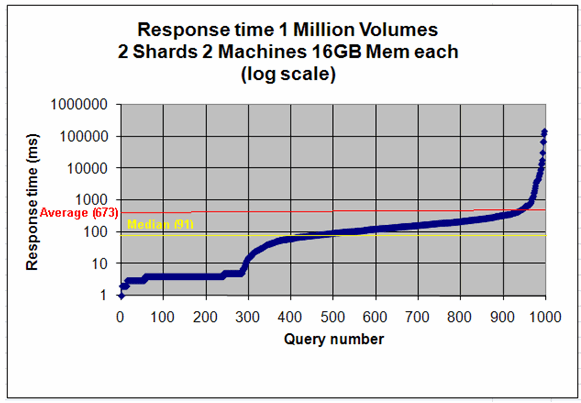
\includegraphics[width=\textwidth]{images/response_time.png}
     \caption{Response Time for a Solr Index with over 1 Million records (Logarithmic Scale)}
\end{figure}


\paragraph{Dynamic Fields in Solr used by Drupal}
As explained, using a combination of field types and field properties a schema can create lots of dynamic configurations for softwares that interact with Solr. In the case of Drupal the Apache Solr Drupal module does not know in advance how the schema should look like because all Drupal sites are differently configured using different content types. The module should be able to cope with most of the use cases that site administrators come up with. If a field name is not found while submitting a new document, the "dynamicFields" type will be used if the name matches any of the patterns. Note that there are restrictions namely that the glob-like pattern in the name attribute must have a "*" only at the start of the end of the field definition. For example, name="\*\_i" will match any field ending in \_i (like myid\_i, z\_i). Longer patterns will be matched first and if equal size patterns both match, the first appearing in the schema will be used.
 
Before starting this work not all of these dynamic fields were provided to the site administrators but with time a list was compiled to meet 99\% of the use cases.  See schema.xml in the project files for the complete list. A small snippet of some of these dynamic fields is included below. The 1st letter indicates the data type and the last letter is 's' for single valued, 'm' for multi-valued.

\inputminted[fontsize=\scriptsize,linenos]{xml}{./code_examples/schema_dynamicfields.xml}
\captionof{listing}{Example of some dynamic field type definitions \label{code:fielddynamicdefinition}}

\noindent In the implementation chapter it will be explained how these dynamic fields are used to create new fields in Solr using Drupal.


\section{Standard Drupal Search}
By default Drupal already ships with a search module that leverages Mysql to its far extent in order to create a search experience that works quite well in smaller scale websites.

In Drupal there is a concept called "cron". These are actions that are executed per set amount of time, for example 30 minutes. Every 30 minutes the designated search actions will index a little set of the selected content, for example 100 pages. This will run until there is no more content to index. Naturally content will change and will need to be re-indexed. This concept is fairly basic and is also the one used for the Apache Solr module. 
However, I'd like to point out that the Search module that is shipped with Drupal differs greatly from the Apache Solr module. 

\paragraph{Advantages} The standard Drupal search module certainly has its advantages. There is, to start with, no extra server/service necessary and it does ship with Drupal core. The basic module also has support for basic text transformations, such as recognition of singular and plural words. It transforms special characters to basic text characters (Similar to the MappingCharFilterFactory in Apache Solr) and it scores items based on their tag where they are embedded in. Examples are H1, H2 and P tags.

\paragraph{Disadvantages} However, it has a hard time handling a big data set. MySQL was not built to be a search engine. Mysql also has its limitations when building a full text search on top of its stack. Drupal also has to comply with the SQL standards so engine specific optimizations cannot be utilized. \footnote{\url{http://dev.mysql.com/doc/refman/4.1/en/fulltext-restrictions.html}}. This leaves the SQL solution with a very restricted set of operators and inherently slow and not scalable in the long haul. 

\paragraph{Conclusion Drupal SQL search} An SQL backend does well in serving a full text search application as long as the number of indexed items stay stable and preferably < 10000 items. \footnote{This number is an estimation, depending on the SQL database application and server configuration this can vary greatly}

\section{Apache Solr Search Integration Drupal Module}
The module found its origin around the end of 2007, at the time of Drupal 5. Its first author was Robert Douglass and lots of other people followed his lead in this initiative. Fast forward and at the moment of writing a Drupal 6 and 7 version exist. When this work started the Drupal 7 version was basically a port of the Drupal 6 version and needed lots of improvements. Acquia sponsors development of this module to ensure continuity and support.

\paragraph{Filtering}
Search facets, also known as filters allow users to refine or sort their search result set. Users can begin with a general search and narrow down the result set as they understand better what content is available on a site.

\begin{wrapfigure}{l}{0.3\textwidth}
\begin{center}
     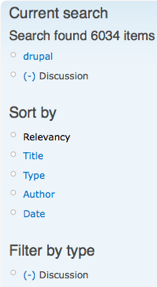
\includegraphics[width=0.25\textwidth]{images/Search_facet_ex_4_by-type-ex-1.png}
     \caption{Filter by Type example. A user clicked on Discussion}\end{center}
\end{wrapfigure}
\paragraph{}
When a user clicks on any term within a filter block it sends a new query to the Apache Solr server and it returns a resultset with the narrowed down results so it only includes content that matches the original query (text search) and the newly selected filter. 
The practice of this narrow-down method is that the user can keep selecting new filters until he finds what he is looking for. The facets can be configured as OR or AND. When the user clicks the minus "(-)" the filter will be removed from the current set and show the results of the search minus that specific filter.

\begin{wrapfigure}{r}{0.60\textwidth}
\begin{center}
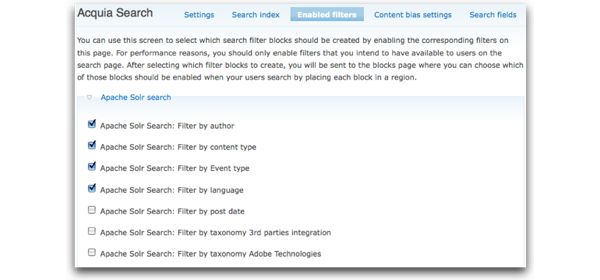
\includegraphics[width=0.60\textwidth]{images/enabled_search_filters_page-1.png}
\caption{Configure the facets}
\end{center}
\end{wrapfigure}

\paragraph{Configuration} When the site creator wants to add more facets it is possible by going to a configuration page. As shown in the picture above. The site creator selects the facets he wants and then configures them in more detail in the block settings. The block configuration page allows you to configure, for example, the number of filters the block displays, how many it displays after clicking the show more link, the title of the block and many more. Some important facets to mention are Author, Content Type, Language, Vocabulary and Dynamic CCK/Field API filters

\paragraph{Content Recommendation}
Apache Solr can also show content suggestions to user that is viewing a specific piece of content. These suggestions are made based on the content of the viewed text. It can be used for suggestions similar to "customers who bought X also liked Y", or simply a list of relevant blog entries. The importance of certain parameters can be adjusted in the bias settings.
\begin{figure}[H]
     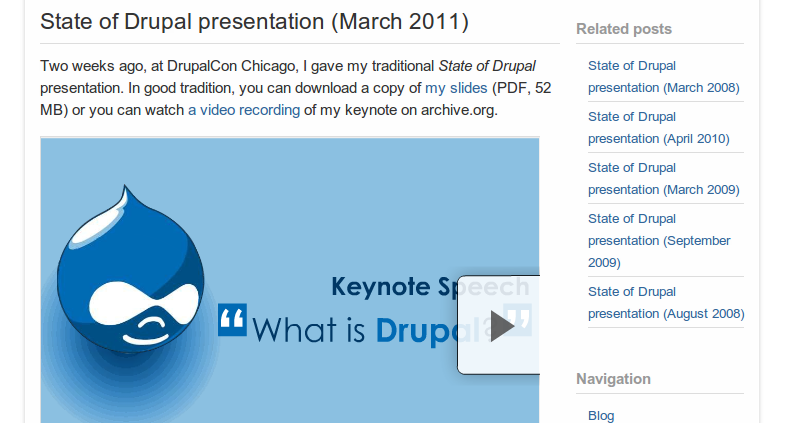
\includegraphics[width=\textwidth]{images/more_like_this.png}
     \caption{Content Recommendations can be seen in the block "Related Posts"}
\end{figure}

\begin{wrapfigure}{l}{0.5\textwidth}
\begin{center}
     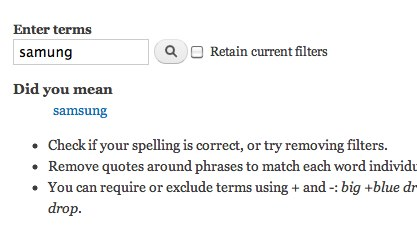
\includegraphics[width=0.5\textwidth]{images/spellchecker.jpg}
     \caption{Spelling correction}
\end{center}
\end{wrapfigure}
\paragraph{Spelling Suggestions}
One of the other features of Apache Solr, and a feature that conquered a lot of hearts in the community was the spellchecker. Similarly to what Google does when you misspell a word it will search in the index for a word similar to your word, but with better/more relevant results.

\paragraph{State of the UI as of September 2011} What is shown below is a snapshot of how the module looked in the backend as of September 2011. There are markers that indicate problem areas. Do take into account that this does not show you any comments made on the code and any internals of the module.
\begin{figure}[H]
     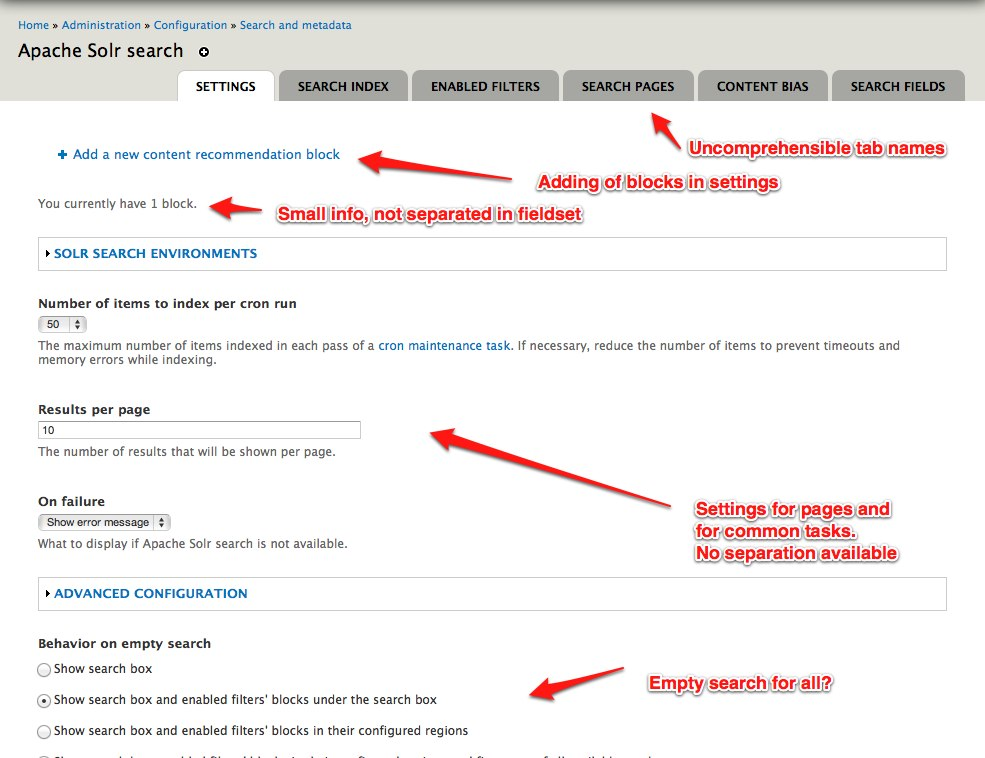
\includegraphics[width=\textwidth]{images/apachesolr_ui_backend_september_2011_1.jpg}
     \caption{UI settings backend, September 2011}
\end{figure}
\paragraph{Summary for the UI settings backend}
\begin{itemize}
\item The tab names are hard to understand. Search bias and/or Search fields are not comprehensible for a first time user.
\item The first like is a link to add a content recommendation block. Surely there must be more important items to appear at the top. 
\item In the settings tab there are global search page settings and ideally those must be generalized so that each search page can use another preset.
\item The use of the "Show search box" appears everywhere and is therefore obsolete.
\end{itemize}

\begin{figure}[H]
     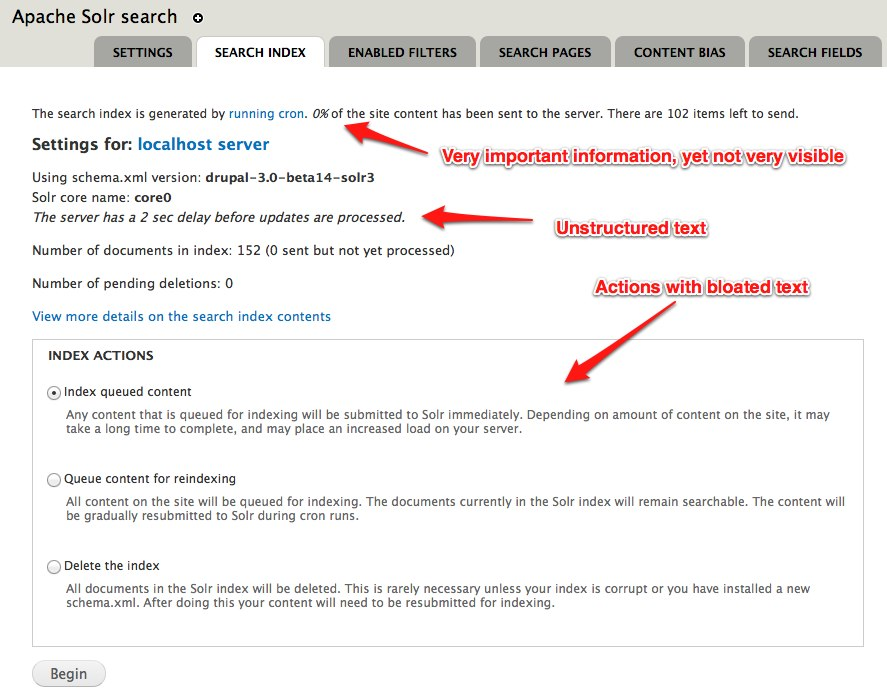
\includegraphics[width=\textwidth]{images/apachesolr_ui_backend_september_2011_2.jpg}
     \caption{UI index report backend, September 2011}
\end{figure}
\paragraph{Summary for the UI report backend}
\begin{itemize}
\item There is information spread out across the whole page. This should be structured and weight should be given to the more important parts.
\item There are 3 types of actions but reading all of them makes you doubt even more about what they do. That should be clarified.
\end{itemize}


\begin{figure}[H]
     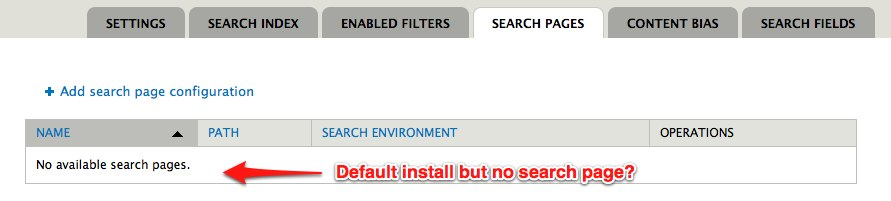
\includegraphics[width=\textwidth]{images/apachesolr_ui_backend_september_2011_3.jpg}
     \caption{UI search pages backend, September 2011}
\end{figure}
\paragraph{Summary for the UI search pages backend}
\begin{itemize}
\item When going to the search pages the first time, the user sees that the list is empty. However, when going to the search in Drupal a new search tab was added. This raises confusion and therefore the core search page (overridden by Apache Solr) should appear in the search pages listing.
\end{itemize}

\begin{figure}[H]
     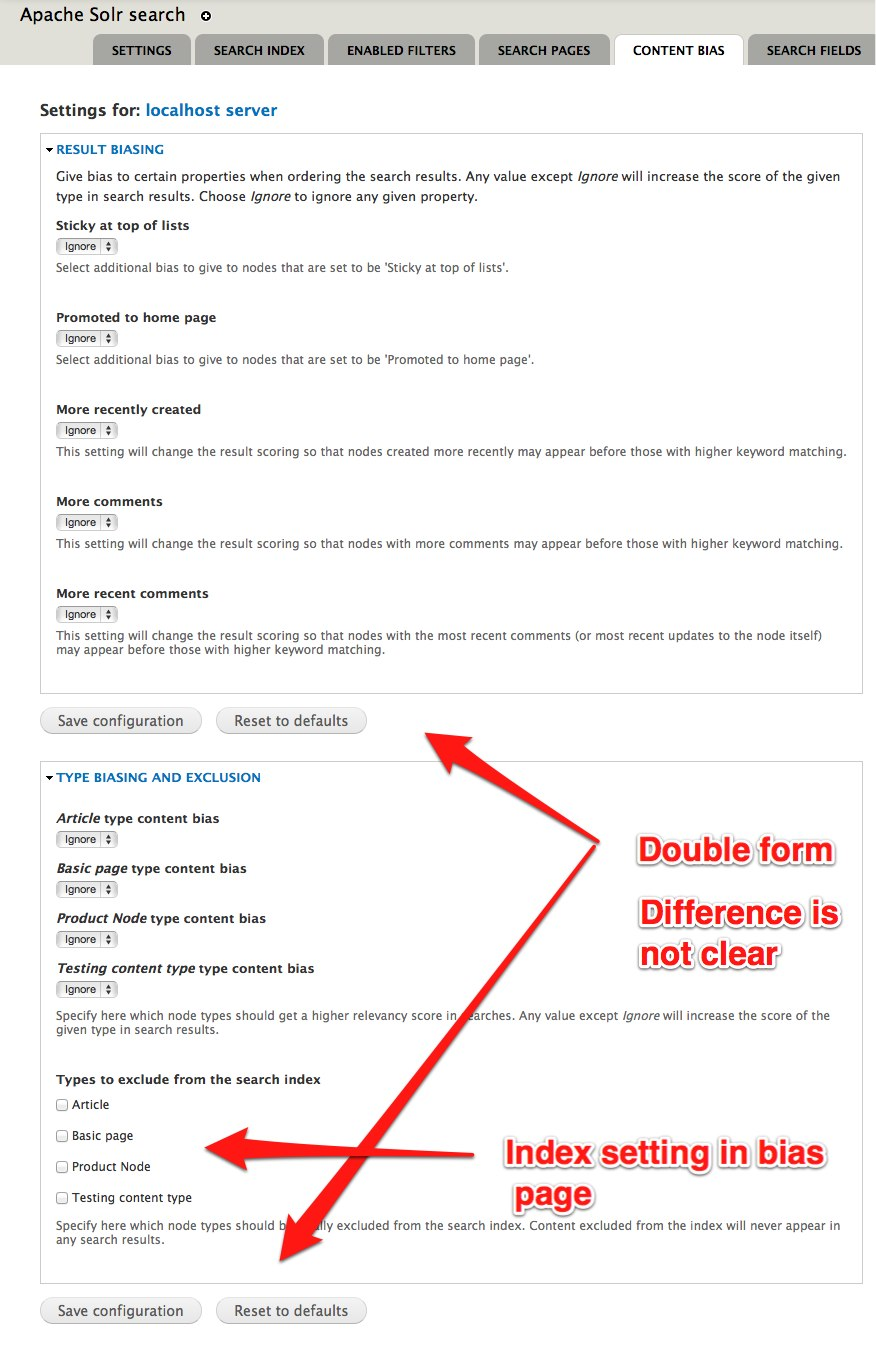
\includegraphics[width=\textwidth/(2)]{images/apachesolr_ui_backend_september_2011_4.jpg}
     \caption{UI for result and index biasing backend, September 2011}
\end{figure}
\paragraph{Summary for the UI index biasing backend}
\begin{itemize}
\item Multiple forms are visible in 1 page. According to the UI standards of Drupal this is a no-go.
\item It also appears there is a settings available, a setting that excludes content types from the index, that should be moved to the index settings. 
\end{itemize}

\paragraph{Architectural challenges}
Drupal and the module were never intended to be built by architects but by people who solve problems, real world problems. Many people worked together to create a cohesive project that is very stable but might not be in agreement with what is taught in classes such as Object Oriented programming, other theories and best practices. A class diagram would be a faulty way to show you the beauty this module has to offer its users since there were hardly object oriented concepts applied to this module that were worthy enough to generate a class-diagram from. Together with Acquia we've set up a list of minimal achievements that should be reached by the end of  February. Some of these items are also issues that were pointed out by other companies or users and they were being put into the issue queue waiting for an answer or a resolution. 

\paragraph{Improvements}
\begin{packed_itemize}
\item UI refactoring to make a better experience \footnote{\url{http://drupal.org/node/1292364}}
\item Support the indexing of multiple entities natively so the module would have an API to index users / terms / ... easily \footnote{\url{http://drupal.org/node/1292364}}
\item Global functions should be context driven.\footnote{\url{http://drupal.org/node/1292364}}
\item Get rid of dependencies in theme layer from core search \footnote{Related to \url{http://drupal.org/node/1314406} (de-duplication)}
\item (Performance) Hooks node\_type, taxonomy and user knocks out our database server \footnote{\url{http://drupal.org/node/592522}}
\item Improve file listing and access control
\item "More like this" blocks should get a delete button \footnote{\url{http://drupal.org/node/1271964}}
\item De-duplicate core and custom search in order to obtain clarity in the code \footnote{\url{http://drupal.org/node/1314406}}
\item Add 1 custom search block with generic render function for custom development
\item The numeric field id should not be used for Solr index field names \footnote{\url{http://drupal.org/node/1161538}}
\item Query type should be adjusted in order to allow different widgets in facetapi \footnote{\url{http://drupal.org/node/1161444}}
\item Change the PHP static to the Drupal function drupal\_static() \footnote{\url{http://drupal.org/node/1334216}}
\item Non-current/valid Node Types are not excluded from index \footnote{\url{http://drupal.org/node/1000532}}
\item Add retain current filters checkbox to custom search page \footnote{\url{http://drupal.org/node/1246422}}
\item Add "retain-filters" param when in facet browsing mode \footnote{\url{http://drupal.org/node/1116792}}
\item Handle one placeholder in a custom search page path which makes the taxonomy sub-module obsolete \footnote{\url{http://drupal.org/node/1294846}}
\item Create tests for the module \footnote{\url{http://drupal.org/node/989398}}
\item Bundle' is not a required field, but the module treats it as such (Evaluate required fields in schema, make non-required if possible) \footnote{\url{http://drupal.org/node/1279164}}
\item Improve Date faceting/date query type (combined with facetapi) \footnote{\url{http://drupal.org/node/1201534}}
\item Facets are currently not linked to the appropriate search page
\item Add clone operation for search environments \footnote{\url{http://drupal.org/node/1292328}}
\item Backport Apache Solr Module to Drupal 6
\end{packed_itemize}

\section{Facetapi Drupal module}
The Facet API module allows site builders to easily create and manage faceted search interfaces. In addition to the UI components that come out of the box, themers and module developers can build their own widgets that can optionally be contributed back to Drupal.org. Facet API works with the core Search, Search API, and Apache Solr Search Integration modules (including Acquia Search) meaning that code and configuration can be reused as-is with the most popular search solutions available to Drupal. It was created by Chris Pliakas and Peter Wolanin specifically for the Drupal 7 version of any search tool. Acquia sponsors development of this module to ensure continuity and support.

\paragraph{State of the UI as of September 2011} What is shown below is a snapshot of how the module looked in the backend and frontend as of September 2011. The markers indicate problem areas. Do take into account that this does not show you any comments made on the programming code and the internals of the module.

Screenshots of the implemented part of facetapi (Drupal 7)
\begin{figure}[H]
     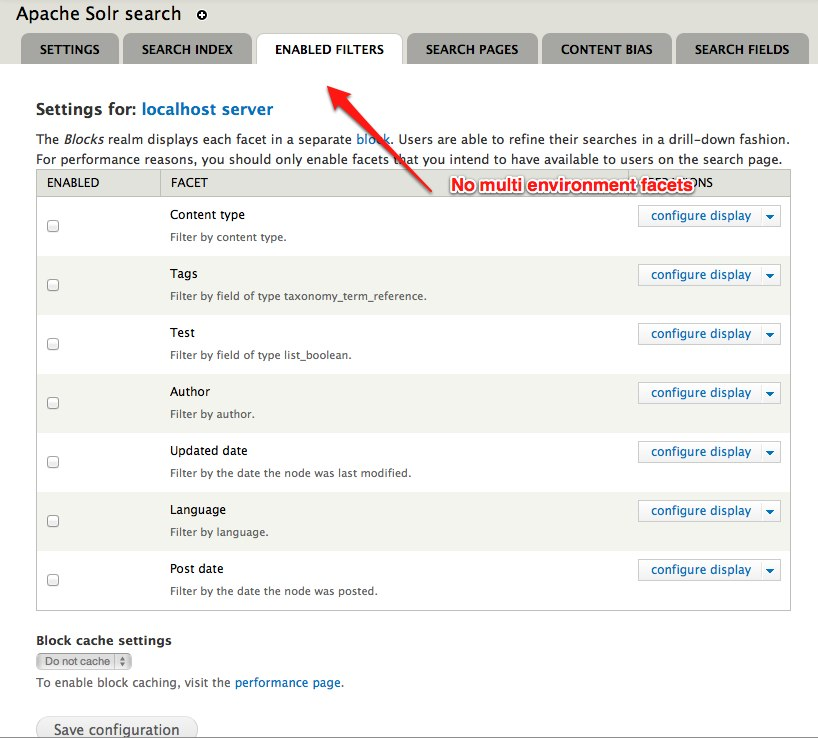
\includegraphics[width=\textwidth]{images/facetapI_ui_september_2011.jpg}
     \caption{Apache Solr Facetapi Integration UI as of September 2011}
\end{figure}
\paragraph{Summary for the UI search pages backend}
\begin{itemize}
\item There was no possibility to easily switch to facets from other environments because one had to make the other environment the default one. This was a huge workaround and had to be fixed.
\end{itemize}

\begin{figure}[H]
     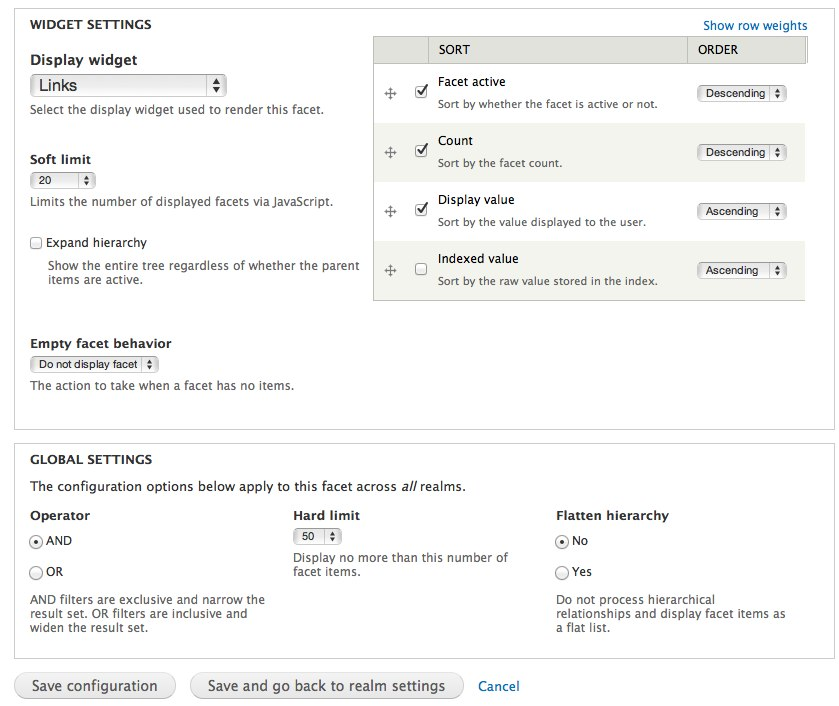
\includegraphics[width=\textwidth]{images/facetapi_ui_facet_september_2011.jpg}
     \caption{Apache Solr Facetapi Integration UI of 1 facet as of September 2011}
\end{figure}
\begin{itemize}
\item The Facet details page was ok in its use and therefore it did not need any further adjustments.
\end{itemize}

\paragraph{Architecture}
As part of the analysis a class diagram was made from the Facet Api code to get a better understanding of the internals. An issue \footnote{\url{http://drupal.org/node/1321136}}was raised in the Facet Api issue queue on \url{drupal.org} for those who prefer to read up in detail.

\begin{figure}[H]
     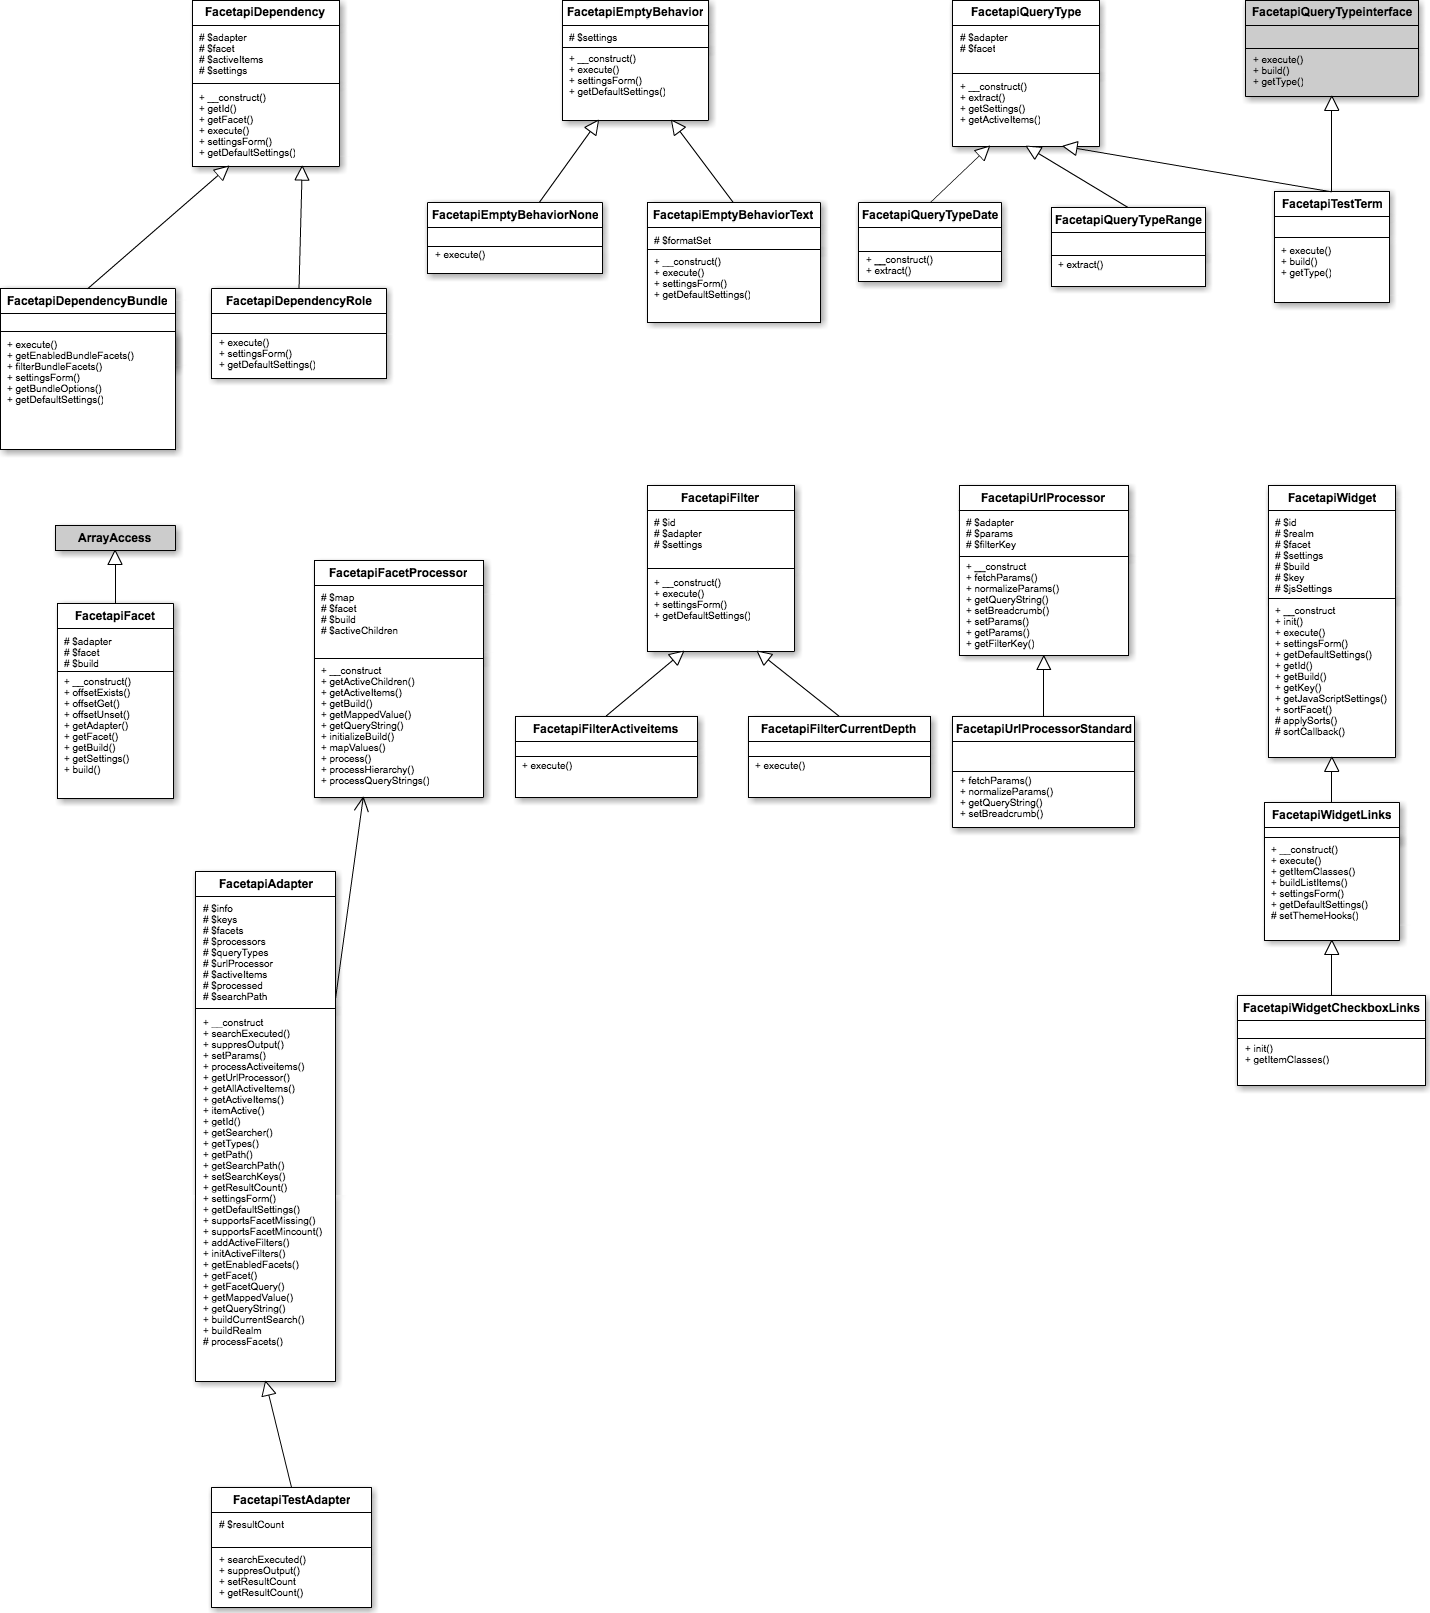
\includegraphics[width=\textwidth]{images/facetapi_classdiagram.png}
     \caption{Extended information about the classes in FacetAPI, September 2011}
\end{figure}

\begin{figure}[H]
     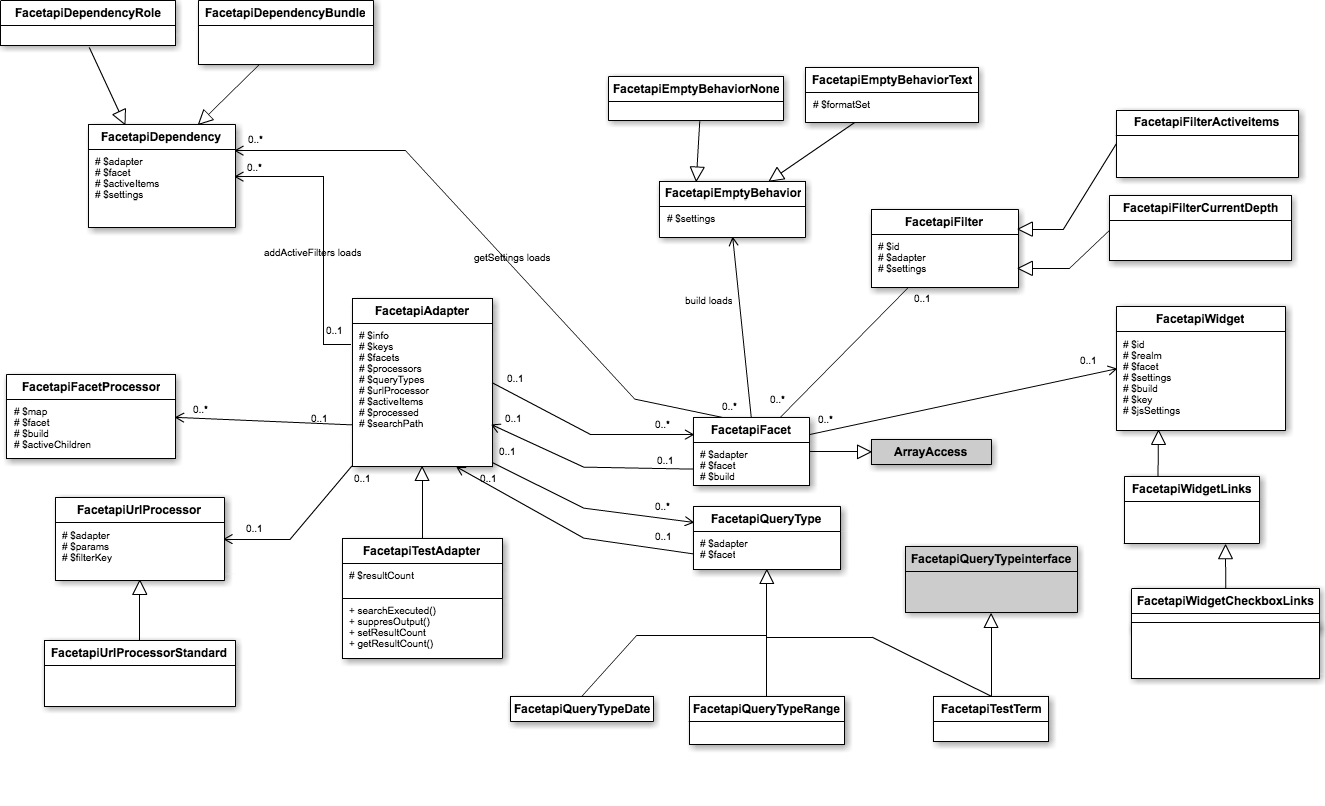
\includegraphics[width=\textwidth]{images/ClassDiagram_facetapi.png}
     \caption{Class Diagram of FacetAPI, September 2011}
\end{figure}

\begin{itemize}
\item There are a number of loop-references between the adapter and its relations. This can possibly be avoided by thinking the architecture through (see the references that have two lines to each other)
\item The variable facet in FacetapiFacet might be a bit too un-descriptive and it looks like it could be renamed to "settings" or "facet\_settings"
\item Doxygen documentation with loads of diagrams and easy to read documentation was generated from this. In addition to the attached images it should make the facetapi module easier to understand. The documentation can be found on \url{http://facetapi.nickveenhof.be}
\end{itemize}

\paragraph{Improvements}
\begin{packed_itemize}
\item Modify "query type" key in facet definition to accept an array \footnote{\url{http://drupal.org/node/1161434}}
\item Make the current search block more configurable \footnote{\url{http://drupal.org/node/593658}}
\item Complete configuration import functionality \footnote{\url{http://drupal.org/node/1147564}}
\item widget.inc change id/class to not reflect the field\_id but a generic one for multisite (line 106) + apachesolr.module line 1860 to remove the id (integer) assumptions
\item Backport Facet Api to Drupal 6
\end{packed_itemize}

\section{Acquia Search for Drupal 6 and 7}
Quote from Dries' blog : "Acquia Search is a hosted search service based on the Software as a Service (SaaS) model. The way it works is that Drupal sites push their content to the search servers hosted by Acquia. We index the content, builds an index, and handle search queries. We provide the search results, facets, and content recommendations to your Drupal site over the network." \footnote{\url{http://buytaert.net/acquia-search-benefits-for-site-administrators}}

As the reader of this paper would have guessed, Acquia Search is built using the Open Source Lucene and Solr distributions from the Apache project. Another quote from Dries' website : "Many organizations simply lack the Java expertise to deploy, manage and scale Java applications or their hosting environment may not accommodate it. Because Acquia Search is a hosted service, it takes away the burden of installation, configuration, and operational duties to keep the software fast, secure and up-to-date."

\paragraph{Architecture}
\begin{figure}[H]
     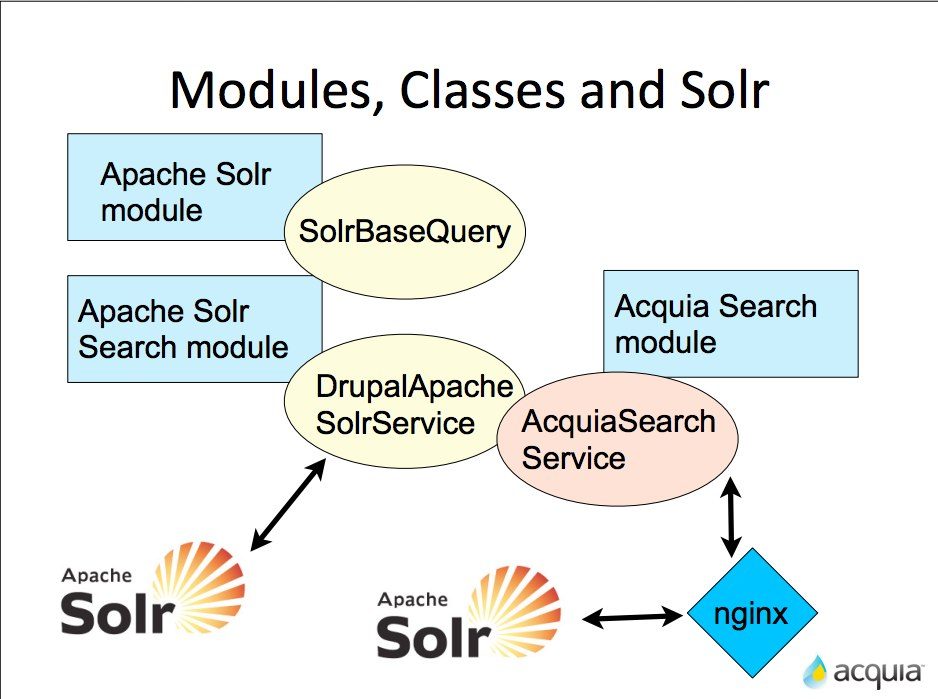
\includegraphics[width=10cm]{images/acquia_solr_classes.jpg}
     \caption{Overview of the classes and services used for Acquia Search at the website's end.}
\end{figure}

Even though the image was not built as a real class diagram it should be clear that there are two classes in the Apache Solr module that are pictured here (yellow). The only important one to cover here is the DrupalApacheSolrService. This class makes it possible to connect to an arbitrary Solr server. When the Acquia Search module is enabled on any website the AcquiaSearchService class extends the DrupalApacheSolrService class and adds the authentication information to all the requests.

The next figure will explain the server side handling of the requests that are being sent to Solr.
\begin{figure}[H]
     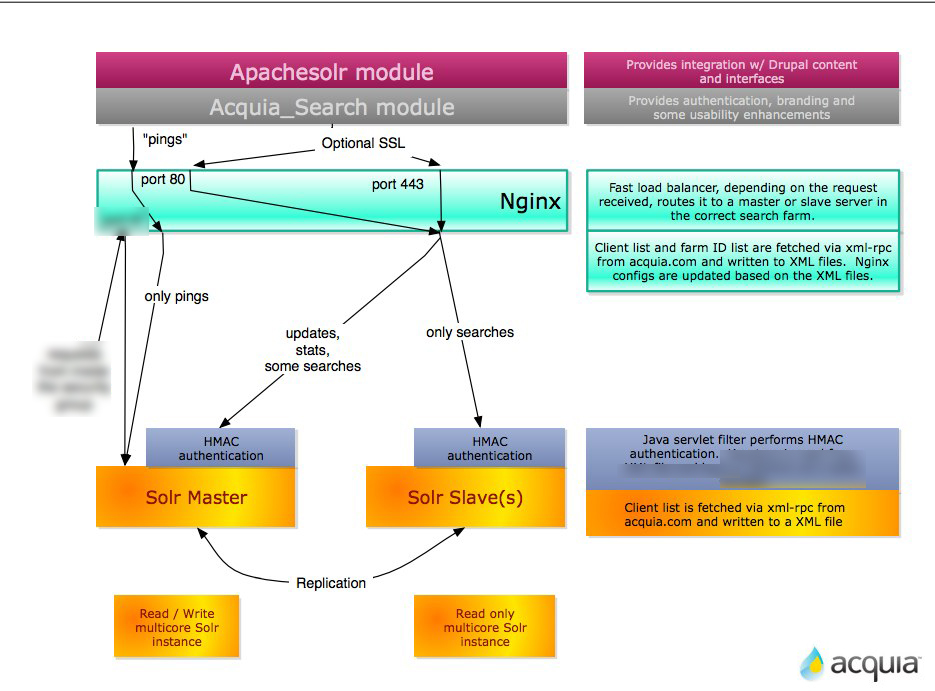
\includegraphics[width=\textwidth]{images/acquia_architecture.jpg}
     \caption{Server Side view of Acquia Search. Certain information has been blurred for confidentiality}
\end{figure}

\paragraph{HMAC authentication filter}
The way it works is that the data is protected during the transport over the web by SSL and to authenticate to the search servers at Acquia an SHA1-HMAC authentication layer is used. This means that the data is encrypted so no man in the middle attack can be exploited. Acquia knows that you have sent the request and will verify, using this SHA1-HMAC authentication, if the data that was sent was not modified. 

This kind of authentication is commonly called a symmetric signature. Using a shared secret the message is signed and also verified as can be seen in the image below.

\begin{figure}[H]
     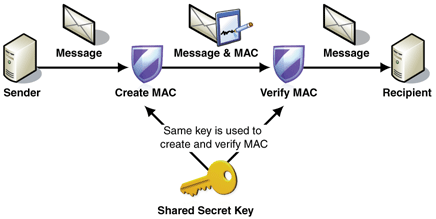
\includegraphics[width=10cm]{images/IC42720.png}
     \caption{Signing a message using a symmetric signature}
\end{figure}

As illustrated in the figure above, signing a message using a symmetric signature involves the following steps:

\begin{itemize}
\item The sender creates a HMAC using a shared secret key and attaches it to the message.
\item The sender sends the message and HMAC to the recipient.
\item The recipient verifies that the HMAC that was sent with the message by using the same shared secret key that was used to create the HMAC.
\end{itemize}

By signing with a shared secret, both data integrity and data origin authenticity are provided for the signed message content. The only downside is that the receiver does not know who exactly wrote the message. He can only verify if it was encrypted with the right shared key. Acquia Search creates a hash from the network identifier (aka the subscription ID from the customer) and generates a secret shared key from this information. Using this derived key and a blob of data it can be easily encoded so the backend is able to verify the authenticity of the message

\inputminted[fontsize=\scriptsize,linenos]{php}{./code_examples/hmac_snippet.php}
\caption{Small excerpt to show how the Client side generates the HMAC message to send back to the Solr Service}

\paragraph{State of Acquia Search}
When the internship started at Acquia there were some blanks left to be filled regarding Acquia Search. Since Solr 3.4 (now 3.5) came out it was only a logical step to convert the Acquia Search service to this newer version of Apache Solr so it could be used in the software as a service ideology that Acquia has. The version that is currently used is Apache Solr 1.4 and is still one of the de facto standards when deploying Solr.

As always,  upgrading does not usually happen overnight without any effort. There are many clients running their active sites from Solr 1.4 and it is not guaranteed that all of these will work perfectly for Solr 3.5. Performance factors are also a key role during this migration. 

As reviewed by the architecture it also needs a confirmed upgrade path for the HMAC authentication, which was written specifically for Solr 1.4 as a Java Servlet.

\paragraph{Improvements}
\begin{itemize}
\item Upgrade the Java Servlet that was written to handle HMAC authentication Solr request to Solr 3.x
\item Test if the Solr 3.x performs better or equally well using the upgraded code and by using existing indexes and a real infrastructure server setup to emulate a real-life situation.
\end{itemize}

\chapter{Implementation}

I started my internship September 22nd in Boston. While being on-site and I learned how Acquia manages processes and works together with the community in order to reach business goals. Also watching them work with a lot of remote employees was already a very valuable lesson. More about this experience can be read in the article [9] I wrote about this. In addition to this I have helped with the creation of some new modules such as Facet Slider [12] and Apachesolr sort UI [13].

As for addressing the public on this subject, I have recently given a presentation ‘Drupal Search’ [6] explaining to more than 60 attendees what was done with the module and where it was heading to in Belgium. Lots of open communication [10] has happened within the community in the Apache Solr Issue Queue. [11] In total I have given 4 presentations with a combined total of more then 200 attendants. Since my involvement with the project there are about 2500 websites using the Drupal 7 version of the module and about 10000 users in total using the module for Drupal 6 and Drupal 7 combined.
  
I’ve contributed several blog posts about this topic and this internship
\begin{itemize}
  \item Presentation about Drupal Search for the DUG group in November 2011. \cite{url10}
  \item Simple guide to install Apache Solr 3.x for Drupal 7 on a unix machine [7]
  \item Adding a custom plugin to the Apache Solr Project [8] 
  \item A Story of an intern at Acquia [9] 
\end{itemize}

Objectives 1, 2 and 3 are in progress and are nearing its completion status. Objective 4, updating the Acquia Search service to the latest stable Apache Solr version, made great progress and is currently being tested by a client of Acquia that required this change. 
Every day there is a daily call with Peter Wolanin to keep the daily objectives clear and to clear out any issues that could block progress.

\section{Apachesolr module for Drupal 6 version 6.x-3.x}
\section{Apachesolr module for Drupal 7 version 7.x-1.0}
\section{Functional requirements}
\subsection{Search Environments}
\subsection{Search pages}
\subsection{Query Object}
\subsection{Apaches Solr Document}
\subsection{Entity layer}
\section{Non-Functional Requirements}
\subsection{User interface}
\subsection{Usability}
\subsection{Performance}
\subsection{Security}
\subsection{Legal}
\include{06_testing}
\chapter{Related Work}
\section{Search Appliances}
\subsection{Elastic Cloud}
\subsection{Sphinx}
\subsection{Some Other}
\section{Drupal Search Solutions}
\subsection{Search API}
\subsection{Drupal Lucene API}
\subsection{Google Search Appliance}

\chapter{Conclusions}
\section{Overview of work}
\section{Reflection on Apache Solr}
\section{Reflection on Drupal 6 and Drupal 7 in regards to search integration}
\section{Future Work}
\subsection{Apache Solr Search Integration}
\subsection{Acquia Search}
\chapter{Acknowledgements}

% Include Glossary
\printglossaries

% Include appendix
\appendix

% Include all appendixes such as references (\includes)
\begin{thebibliography}{99}
	\bibitem{book_solr3}
		Apache Solr 3 Enterprise Search Server RAW Book \& eBook | Packt Publishing Technical \& IT Book and eBook Store\\
		\emph{\url{http://www.packtpub.com/apache-solr-3-enterprise-search-server/book}}
	\bibitem{url2}
		\emph{\url{http://people.apache.org/~hossman/apachecon2009us/apache-solr-out-of-the-box.pdf people.apache.org/~hossman/apachecon2009us/apache-solr-out-of-the-box.pdf}}
	\bibitem{url3}
		[solr-user] Limit number of docs that can be indexed (security) - Search by Lucid Imagination\\
		\emph{\url{http://www.lucidimagination.com/search/document/23d645855e8417a1/limit_number_of_docs_that_can_be_indexed_security}}
	\bibitem{url4}
		\emph{\url{https://acquia.com/sites/default/files/blog/DC-Chicago-2011-Solr-Chops-v3.pdf}}
	\bibitem{url5}
	 	FieldCollapsing \- Solr Wiki\\
		\emph{\url{http://wiki.apache.org/solr/FieldCollapsing}}
	\bibitem{url6}
		Issues for Apache Solr Search Integration | drupal.org\\
		\emph{\url{http://drupal.org/project/issues/apachesolr}}
	\bibitem{url7}
		CoreAdmin \- Solr Wiki\\
		\emph{\url{http://wiki.apache.org/solr/CoreAdmin}}
	\bibitem{url8}
		Double ellipses on search snippets. | drupal.org\\
		\emph{\url{http://drupal.org/node/1264786}}
	\bibitem{url9}
		Dynamic queries | drupal.org\\
		\emph{\url{http://drupal.org/node/310075}}
	\bibitem{url10}
		[\#SOLR-232] let Solr set request headers (for logging) - ASF JIRA\\
		\emph{\url{https://issues.apache.org/jira/browse/SOLR-232}}
	\bibitem{url11}
	 	[\#SOLR-2452] rewrite solr build system - ASF JIRA\\
		\emph{\url{https://issues.apache.org/jira/browse/SOLR-2452}}
	\bibitem{url12}
		Compiling with Ant – genoviz\\
		\emph{\url{http://sourceforge.net/apps/trac/genoviz/wiki/Compiling with Ant}}
	\bibitem{url13}
		Update war file for report reader - Attias\\
		\emph{\url{http://attias.myftp.org/attias/index.php/Update_war_file_for_report_reader}}
	\bibitem{url14}
		solr at master from distilledmedia/munin-plugins \- GitHub\\
		\emph{\url{https://github.com/distilledmedia/munin-plugins/tree/master/solr}}
	\bibitem{url15}
		Date-boosting Solr / Drupal search results | Metal Toad Media\\
		\emph{\url{http://www.metaltoad.com/blog/date-boosting-solr-drupal-search-results}}
	\bibitem{url16}
		Major Solr 4 Highlights | Javalobby\\
		\emph{\url{http://java.dzone.com/videos/major-solr-4-highlights}}
	\bibitem{url17}
		Solr Black Belt Pre\-conference \\
		\emph{\url{http://www.slideshare.net/erikhatcher/solr-black-belt-preconference}}
	\bibitem{url18}
		Some tips for Solr tuning - Vizrt forum\\
		\emph{\url{http://forum.vizrt.com/showthread.php?t=5177}}
	\bibitem{url19}
		Getting started faster with LucidWorks for Solr \\
		\emph{\url{http://www.slideshare.net/LucidImagination/improving-findability}}
	\bibitem{url20}
		Spatial Indexes: Solr — Derick Rethans \\
		\emph{\url{http://derickrethans.nl/spatial-indexes-solr.html}}
	\bibitem{url21}
		Using Apache Access Logs with JMeter \\
		\emph{\url{http://minaret.biz/tips/jmeter.html}}
	\bibitem{url22}
		Jmeter used to playback Apache access logs to generate live-like server load | artur.ejsmont.org \\
		\emph{\url{http://artur.ejsmont.org/blog/content/jmeter-used-to-playback-apache-access-logs-to-generate-live-like-server-load}}
	\bibitem{url23}
		Drupal Patching, Committing, and Squashing with Git | RandyFay.com\\
		\emph{\url{http://randyfay.com/node/97}}
	\bibitem{url24}
		svn get last commit message - Alec\'s Web Log \\
		\emph{\url{http://www.alecjacobson.com/weblog/?p=2042}}
	\bibitem{url25}
		GitX - See It \\
		\emph{\url{http://gitx.frim.nl/seeit.html}}
	\bibitem{url26}
		Add SSh key to Server \\
		\emph{\url{http://oreilly.com/pub/h/66}}
	\bibitem{url27}
		Maintaining patch series with Stacked GIT: a walk-through | drupal.org \\
		\emph{\url{http://drupal.org/node/337933}}
	\bibitem{url28}
		Git Best Practices: Upgrading the Patch Process | Lullabot \\
		\emph{\url{http://www.lullabot.com/articles/git-best-practices-upgrading-patch-process}}
	\bibitem{url29}
		Issues for Facet API | drupal.org\\
		\emph{\url{http://drupal.org/project/issues/facetapi?categories=All}}
	\bibitem{url35}
		Issues for Drupal core | drupal.org\\
		\emph{\url{http://drupal.org/project/issues/drupal?status=1&categories=bug&version=7.x}}
	\bibitem{url36}
		\emph{\url{http://bxl2011.drupaldays.org/sites/default/files/Search API Presentation.pdf}}
	\bibitem{url37}
		Interface text | drupal.org\\
		\emph{\url{http://drupal.org/node/604342}}
	\bibitem{url38}
		Backpack: Debugging Drupal\\
		\emph{\url{https://ratatosk.backpackit.com/pub/1836982-debugging-drupal}}
	\bibitem{url39}
		Using apachebench (ab) with Drupal 7 to load test site with authenticated users | Midwestern Mac, LLC \\
		\emph{\url{http://www.midwesternmac.com/blogs/jeff-geerling/using-apachebench-ab-drupal-7}}
	\bibitem{url40}
		Apache Bench (ab) | drupal.org\\
		\emph{\url{http://drupal.org/node/659974}}
	\bibitem{url41}
		Supercolliding a PHP array\\
		\emph{\url{http://nikic.github.com/2011/12/28/Supercolliding-a-PHP-array.html}}
	\bibitem{url42}
		Awesome Testing Party Cheat Sheet\\
		\emph{\url{http://dmitrizone.com/Awesome Testing Party Cheat Sheet.html}}
	\bibitem{url44}
		Miscellaneous Simpletest Tips | drupal.org\\
		\emph{\url{http://drupal.org/node/30011}}
	\bibitem{url45}
		Apache Solr search integration module | drupal.org\\
		\emph{\url{http://drupal.org/project/apachesolr}}
	\bibitem{url46}
		Facet Api Module |  drupal.org\\
		\emph{\url{http://drupal.org/project/facetapi}}
	\bibitem{url47}
		Acquia Search product information\\
		\emph{\url{http://acquia.com/productsservices/acquia-search}}
	\bibitem{url48}
		Apache Solr project page\\
		\emph{\url{http://lucene.apache.org/solr/}}
	\bibitem{url54}
		Drupal.org user profile of Nick\_vh (Nick Veenhof)\\
		\emph{\url{http://drupal.org/user/122682/track}}
	\bibitem{url55}
		Issue queue of Apache Solr search integration module\\
		\emph{\url{http://drupal.org/project/issues/apachesolr}}
	\bibitem{url56}
		Facet Api Slider module project page\\
		\emph{\url{http://drupal.org/project/facetapi_slider}}
	\bibitem{url57}
		Apache Solr Sort UI project page\\
		\emph{\url{http://drupal.org/project/apachesolr_sort}}
	\bibitem{url59}
		Acquia Network product information\\
		\emph{\url{http://www.acquia.com/products-services/acquia-network}}
	\bibitem{google_paper}
		Brin, S. and L.~Page (1998).
		\newblock The anatomy of a large-scale hypertextual web search engine.
		\newblock{\em Computer Networks and ISDN Systems\/}~{\em 30}, 107--117.\\
		\emph{\url{http://infolab.stanford.edu/\textasciitilde backrub/google.html}}
	\bibitem{drupal_license}
		Drupal License\\
		\emph{\url{http://drupal.org/licensing/faq\#q1}}
	\bibitem{apache_license}
		Apache License\\
		\emph{\url{http://en.wikipedia.org/wiki/Apache_License}}

http://msdn.microsoft.com/en-us/library/ff648434.aspx
\end{thebibliography}



\backmatter

% Optionally a list of figures and/or tables
\listoffigures
\listoftables

% lege pagina (!!)
\newpage

% kaft

\end{document}
